\chapter{Random Variables}
\addtolength{\topmargin}{-0.9pt}

\section{Basic Concepts}

\begin{definition}[Random Variable]
A \emph{random variable} is a function 
\[
X : \samplespace \to \mathbb{R}
\]
from the sample space \( \samplespace \) of an experiment to the set of real numbers \( \mathbb{R} \).
\end{definition}

\begin{eg}
Suppose we choose \(3\) elements from the set \(\{1,2,\dots,6\}\) uniformly at random.  
Then the sample space is 
\[
\samplespace = \{ \{1,2,3\}, \{1,2,4\}, \dots, \{4,5,6\} \},
\]
and 
\[
|\samplespace| = \binom{6}{3} = 20.
\]

\begin{enumerate}[label=(\alph*)]
    \item Define a random variable 
    \[
    X : \samplespace \to \mathbb{R}, \quad X(\{a,b,c\}) = \max(a,b,c).
    \]
    Then 
    \[
    \text{Range}(X) = \{3,4,5,6\}.
    \]
    
    \item Define another random variable 
    \[
    Y : \samplespace \to \mathbb{R}, \quad Y(\{a,b,c\}) = \frac{a+b+c}{3}.
    \]
    Then 
    \[
    \text{Range}(Y) = \{2, 2.5, 3, 3.5, 4, 4.5, 5\}.
    \]
\end{enumerate}
\end{eg}

\begin{eg}
Consider all permutations of the numbers \(1,2,3,4,5\).  
Define the random variable
\[
Z(\pi) = \#\{ i \in \{1,\dots,5\} : \pi(i) \neq i \},
\]
the number of elements that are \emph{not} in their original position (i.e., the number of displaced elements).

For example:
\[
Z(12345) = 0, \qquad Z(12453) = 2.
\]
\end{eg}

\begin{eg}
You have \(5\) cameras, of which \(2\) work and \(3\) do not.  
You mix them up and test them one by one until you find a working one.  
Let the random variable \(W\) be the number of cameras tested.

Then the range of \(W\) is
\[
\text{Range}(W) = \{1,2,3\},
\]
since the first working camera could appear in the first, second, or third test at most (after testing 3 failed ones, you are guaranteed a working one next).
\end{eg}

\begin{definition}[Probability Mass Function]
Let \(X\) be a discrete random variable with range
\[
R_X = \{x_1, x_2, x_3, \ldots\},
\]
where \(R_X\) is finite or countably infinite.  
The \emph{probability mass function (PMF)} of \(X\) is the function
\[
p_X(x) = \Pr(X = x), \quad x \in \mathbb{R}.
\]
The PMF satisfies:
\[
p_X(x) \ge 0 \quad \forall x, 
\qquad \sum_{x \in R_X} p_X(x) = 1.
\]
\end{definition}

\begin{eg}
Continuing from Example 1, let \( X = \max(a,b,c) \).  
To find its PMF, note that:

\begin{itemize}
    \item For \(X = 3\): the only possible subset is \(\{1,2,3\}\), so \(\Pr(X=3) = \frac{1}{20}\).
    \item For \(X = 4\): we must have \(4\) included and the other two from \(\{1,2,3\}\), giving \(\binom{3}{2} = 3\) subsets, so \(\Pr(X=4) = \frac{3}{20}\).
    \item For \(X = 5\): we must have \(5\) included and the other two from \(\{1,2,3,4\}\), giving \(\binom{4}{2} = 6\) subsets, so \(\Pr(X=5) = \frac{6}{20}\).
    \item For \(X = 6\): we must have \(6\) included and the other two from \(\{1,2,3,4,5\}\), giving \(\binom{5}{2} = 10\) subsets, so \(\Pr(X=6) = \frac{10}{20} = \frac{1}{2}\).
\end{itemize}

Hence,
\[
f_X(x) =
\begin{cases}
\dfrac{1}{20}, & x = 3, \\[6pt]
\dfrac{3}{20}, & x = 4, \\[6pt]
\dfrac{6}{20}, & x = 5, \\[6pt]
\dfrac{10}{20}, & x = 6, \\[6pt]
0, & \text{otherwise.}
\end{cases}
\]

We can verify normalization:
\[
\frac{1 + 3 + 6 + 10}{20} = \frac{20}{20} = 1.
\]
\end{eg}

\begin{eg}
You have \(5\) cameras, of which \(2\) work and \(3\) do not.  
You mix them up and test them one by one until you find a working one.  
Let the random variable \(W\) be the number of cameras tested.

Then the range of \(W\) is
\[
\text{Range}(W) = \{1,2,3\},
\]
since the first working camera could appear in the first, second, or third test at most (after testing \(3\) failed ones, you are guaranteed a working one next).

We can compute the probability mass function \(p_W(k) = P(W = k)\) as follows.

\[
f_W(w) =
\begin{cases}
\dfrac{2}{5}, & w = 1, \\[1em]
\dfrac{3}{5}\cdot\dfrac{2}{4} = \dfrac{3}{10}, & w = 2, \\[1em]
\dfrac{3}{5}\cdot\dfrac{2}{4} = \dfrac{6}{20}, & w = 3, \\[1em]
0, & \text{otherwise.}
\end{cases}
\]

\textbf{Verification:}
\[
\frac{2}{5} + \frac{3}{10} + \frac{6}{20} = 1,
\]
so the PMF is valid.
\end{eg}

\begin{eg}
    Throw a 4-sided die until you get a ``3''.  
    Let the random variable \( X \) be the number of throws required to get the first ``3''.  

    \[
    \text{Range}(X) = \mathbb{N} = \{1, 2, 3, \dots\}.
    \]

    The probability of success (getting a ``3'') on any single throw is \( p = \dfrac{1}{4} \),  
    and the probability of failure is \( q = 1 - p = \dfrac{3}{4} \).

    \begin{enumerate}[label=(\alph*)]
        \item For \( X = 8 \):
        \[
        f_X(8) = P(X = 8) = q^{8-1}p = \left(\dfrac{3}{4}\right)^{7} \left(\dfrac{1}{4}\right).
        \]

        \item In general, for the geometric distribution:
        \[
        f_X(k) = P(X = k) = q^{k-1}p = 
        \left( \dfrac{3}{4} \right)^{k-1} 
        \left( \dfrac{1}{4} \right),
        \quad k = 1, 2, 3, \dots
        \]

        \item To verify that \( f_X \) is a valid PMF:
        \[
        \sum_{k=1}^{\infty} f_X(k)
        = \sum_{k=1}^{\infty} \left( \dfrac{3}{4} \right)^{k-1} 
        \left( \dfrac{1}{4} \right)
        = \dfrac{1}{4} \sum_{k=0}^{\infty} 
        \left( \dfrac{3}{4} \right)^k
        = \dfrac{1}{4} \cdot \dfrac{1}{1 - \frac{3}{4}}
        = 1.
        \]
    \end{enumerate}
\end{eg}


\section{More on discrete random variables}

\begin{definition}[Cumulative Distribution Function]
    The \emph{cumulative distribution function (CDF)} of a random variable \( X \) is defined as
    \[
        F_X(x) = P(X \le x), \quad \forall x \in \mathbb{R}.
    \]
\end{definition}

\begin{eg}
    Let \(Y\) be a discrete random variable with probability mass function \(f_Y(y)\) given by

    \[
    f_Y(y) =
    \begin{cases}
        \dfrac{1}{15}, & y = -1, \\[3mm]
        \dfrac{3}{15}, & y = 0, \\[3mm]
        \dfrac{4}{15}, & y = 2, \\[3mm]
        \dfrac{2}{15}, & y = 6, \\[3mm]
        \dfrac{5}{15}, & y = 10, \\[3mm]
        0, & \text{otherwise}.
    \end{cases}
    \]

    \begin{enumerate}[label=(\alph*)]
        \item Verify that this is a valid PMF:  
        \[
        \frac{1}{15} + \frac{3}{15} + \frac{4}{15} + \frac{2}{15} + \frac{5}{15} = \frac{15}{15} = 1.
        \]

        \item Compute the CDF \(F_Y(y) = P(Y \le y)\):
        \[
        F_Y(y) =
        \begin{cases}
            0, & y < -1, \\[1mm]
            \frac{1}{15}, & -1 \le y < 0, \\[2mm]
            \frac{4}{15}, & 0 \le y < 2, \\[2mm]
            \frac{8}{15}, & 2 \le y < 6, \\[2mm]
            \frac{10}{15}, & 6 \le y < 10, \\[2mm]
            1, & y \ge 10.
        \end{cases}
        \]
    \end{enumerate}
\end{eg}


\begin{remark}
The probability mass function (PMF) and the cumulative distribution function (CDF) describe a random variable in related but distinct ways.

\begin{center}
\renewcommand{\arraystretch}{1.2}
\begin{tabular}{c|ccc}
\hline
\textbf{Aspect} & \textbf{PMF} & \textbf{CDF} \\ \hline
Symbol & $p_X(x)$ & $F_X(x)$ \\ \hline
Definition & $p_X(x)=P(X=x)$ & $F_X(x)=P(X\le x)$ \\ \hline
Domain & Discrete $x$ & Real $x$ \\ \hline
Range & $[0,1]$ & $[0,1]$ \\ \hline
Relation & $F_X(x)=\sum_{t\le x}p_X(t)$ & $p_X(x)=F_X(x)-F_X(x^-)$ \\ \hline
Nature & Stepwise (non-continuous) & Non-decreasing, right-continuous \\ \hline
\end{tabular}
\end{center}
\end{remark}


% exmaples, check phones for picture. 



\begin{exercise}
$X$ is uniform over $[0,5] \cup [10,20]$. Find $F_X(x)$ and draw it.
\end{exercise}

\begin{proof}
The total length of the support is $5 + 10 = 15$.

The cumulative distribution function is:
\[
F_X(x) = \begin{cases}
0 & x < 0 \\
\frac{x}{15} & 0 \leq x < 5 \\
\frac{5}{15} = \frac{1}{3} & 5 \leq x < 10 \\
\frac{5 + (x-10)}{15} = \frac{x-5}{15} & 10 \leq x < 20 \\
1 & x \geq 20
\end{cases}
\]

\begin{center}
\begin{tikzpicture}
\begin{axis}[
    axis lines = center,
    xlabel = {$x$},
    ylabel = {$F_X(x)$},
    xmin=-1, xmax=22,
    ymin=-0.1, ymax=1.2,
    xtick={0,5,10,20},
    ytick={0,0.333,1},
    yticklabels={0,$\frac{1}{3}$,1},
    width=10cm,
    height=6cm
]
\addplot[domain=-1:0, blue, thick] {0};
\addplot[domain=0:5, blue, thick] {x/15};
\addplot[domain=5:10, blue, thick] {1/3};
\addplot[domain=10:20, blue, thick] {(x-5)/15};
\addplot[domain=20:22, blue, thick] {1};
\end{axis}
\end{tikzpicture}
\end{center}
\end{proof}

\begin{exercise}
$Y$ has range $[0,10] \cup [20,25]$. It is uniform over $[0,10]$ and uniform over $[20,25]$ with $P(10 \leq Y \leq 25) = 3 \cdot P(0 \leq Y \leq 10)$. Find $F_Y$
$X$ is uniform over $[0,5] \cup [10,20]$. Find $f_X(x)$ and draw it.
\end{exercise}

\begin{proof}
The total length of the support is $(5 - 0) + (20 - 10) = 15$.
For a uniform distribution, the pdf $f_X(x)$ is $1/(\text{Total Length})$ over the support, and $0$ elsewhere.
\[
f_X(x) = \begin{cases}
\frac{1}{15} & 0 \leq x \leq 5 \\
\frac{1}{15} & 10 \leq x \leq 20 \\
0 & \text{otherwise}
\end{cases}
\]

\begin{center}
\begin{tikzpicture}
\begin{axis}[
    axis lines = center,
    xlabel = {$x$},
    ylabel = {$f_X(x)$},
    xmin=-1, xmax=22,
    ymin=-0.05, ymax=0.15,
    xtick={0,5,10,20},
    ytick={0.0667},
    yticklabels={$\frac{1}{15}$},
    width=10cm,
    height=5cm
]
\addplot[blue, thick, domain=-1:0] {0};
\addplot[blue, thick, domain=0:5] {1/15};
\addplot[blue, thick, domain=5:10] {0};
\addplot[blue, thick, domain=10:20] {1/15};
\addplot[blue, thick, domain=20:22] {0};
% Vertical lines to close the boxes
\draw[blue, thick] (axis cs:0,0) -- (axis cs:0,0.0667);
\draw[blue, thick] (axis cs:5,0.0667) -- (axis cs:5,0);
\draw[blue, thick] (axis cs:10,0) -- (axis cs:10,0.0667);
\draw[blue, thick] (axis cs:20,0.0667) -- (axis cs:20,0);
\end{axis}
\end{tikzpicture}
\end{center}
\end{proof}

\begin{exercise}
$Y$ has range $[0,10] \cup [20,25]$. It is uniform over $[0,10]$ and uniform over $[20,25]$ with $P(20 \leq Y \leq 25) = 3 \cdot P(0 \leq Y \leq 10)$. Find $F_Y(y)$.
\end{exercise}

\begin{proof}
Let $P(0 \leq Y \leq 10) = p_1$ and $P(20 \leq Y \leq 25) = p_2$.
Given: $p_1 + p_2 = 1$ and $p_2 = 3p_1$.
Substituting gives $p_1 + 3p_1 = 1 \implies 4p_1 = 1 \implies p_1 = \frac{1}{4}$ and $p_2 = \frac{3}{4}$.

We find the pdf $f_Y(y)$ heights.
For $0 \leq y \leq 10$ (length 10): $\int_0^{10} c_1 \, dy = p_1 \implies 10 c_1 = \frac{1}{4} \implies c_1 = \frac{1}{40}$.
For $20 \leq y \leq 25$ (length 5): $\int_{20}^{25} c_2 \, dy = p_2 \implies 5 c_2 = \frac{3}{4} \implies c_2 = \frac{3}{20}$.

Now, we find the CDF $F_Y(y) = \int_{-\infty}^y f_Y(t) \, dt$:
\[
F_Y(y) = \begin{cases}
0 & y < 0 \\
\int_0^y \frac{1}{40} \, dt = \frac{y}{40} & 0 \leq y < 10 \\
F_Y(10) = \frac{10}{40} = \frac{1}{4} & 10 \leq y < 20 \\
F_Y(20) + \int_{20}^y \frac{3}{20} \, dt = \frac{1}{4} + \frac{3(y-20)}{20} & 20 \leq y < 25 \\
F_Y(25) = \frac{1}{4} + \frac{3(25-20)}{20} = \frac{1}{4} + \frac{15}{20} = 1 & y \geq 25
\end{cases}
\]
\end{proof}

\begin{exercise}
Random variable $Z$ has range $[0,4]$ with $f_Z(z) = Cz^2$. Find $c$.
\begin{center}
\begin{tikzpicture}
\begin{axis}[
    axis lines = center,
    xlabel = {$z$},
    ylabel = {$f_Z(z)$},
    xmin=-0.5, xmax=4.5,
    ymin=-0.05, ymax=0.9,
    xtick={0,4},
    ytick={0.75},
    yticklabels={$\frac{3}{4}$},
    width=8cm,
    height=6cm,
    samples=100
]
\addplot[blue, thick, domain=0:4] {(3/64)*x^2};
\node[above left] at (axis cs:3, { (3/64)*3^2 }) {$f_Z(z) = Cz^2$};
\addplot[dashed, domain=0:4, opacity=0.5] coordinates {(4,0) (4, 0.75)};
\end{axis}
\end{tikzpicture}
\end{center}
\end{exercise}

\begin{proof}
For $f_Z(z)$ to be a valid pdf, its integral over its range $[0,4]$ must be 1.
\[
\int_0^4 Cz^2 \, dz = 1
\]
\[
C \left[ \frac{z^3}{3} \right]_0^4 = 1
\]
\[
C \left( \frac{4^3}{3} - \frac{0^3}{3} \right) = 1
\]
\[
C \left( \frac{64}{3} \right) = 1 \implies c = \frac{3}{64}
\]
(The peak value at $z=4$ is $f_Z(4) = \frac{3}{64}(4^2) = \frac{3 \cdot 16}{64} = \frac{48}{64} = \frac{3}{4}$.)
\end{proof}

\begin{exercise}
Random variable $W$ has the following pdf. Find $f_W(w)$.
\begin{center}
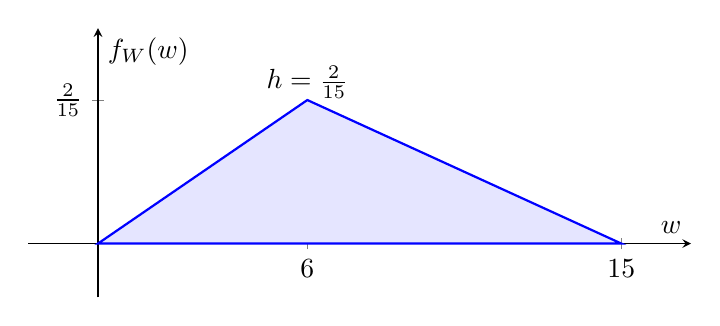
\begin{tikzpicture}
\begin{axis}[
    axis lines = center,
    xlabel = {$w$},
    ylabel = {$f_W(w)$},
    xmin=-2, xmax=17,
    ymin=-0.05, ymax=0.2,
    xtick={0,6,15},
    ytick={0.1333},
    yticklabels={$\frac{2}{15}$},
    width=10cm,
    height=5cm
]
\addplot[blue, thick, fill=blue!10] coordinates {(0,0) (6, 0.1333) (15,0) (0,0)} -- cycle;
\node at (axis cs:6, 0.15) {$h = \frac{2}{15}$};
\end{axis}
\end{tikzpicture}
\end{center}
\end{exercise}

\begin{proof}
The pdf is a triangle with base $b=15$. The area must be 1, so $\frac{1}{2} \cdot 15 \cdot h = 1$, which gives the height $h = \frac{2}{15}$ at the peak $w=6$.

We find the equations for the two lines:
\begin{itemize}
    \item \textbf{Line 1 ($0 \leq w < 6$):} Passes through $(0,0)$ and $(6, 2/15)$.
    Slope $m_1 = \frac{2/15}{6} = \frac{1}{45}$.
    Equation: $f_W(w) = \frac{1}{45}w$.
    
    \item \textbf{Line 2 ($6 \leq w \leq 15$):} Passes through $(6, 2/15)$ and $(15, 0)$.
    Slope $m_2 = \frac{0 - 2/15}{15 - 6} = -\frac{2}{135}$.
    Using point $(15,0)$: $f_W(w) = -\frac{2}{135}(w - 15) = \frac{2}{9} - \frac{2}{135}w$.
\end{itemize}

\[
f_W(w) = \begin{cases}
\frac{1}{45}w & 0 \leq w < 6 \\
\frac{2}{9} - \frac{2}{135}w & 6 \leq w \leq 15 \\
0 & \text{otherwise}
\end{cases}
\]
\end{proof}



\begin{exercise}
\begin{center}
\begin{tikzpicture}[scale=0.6]
    % Axes
    \draw[->] (0,0) -- (17,0) node[right] {$x$};
    \draw[->] (0,0) -- (0,5) node[above] {$f_X(x)$};
    
    % Piecewise PDF
    \draw[thick] (0,0) -- (6,3); % sloped part
    \draw[thick] (6,3) -- (15,3); % flat part

    % Labels
    \node[below] at (6,0) {6};
    \node[below] at (15,0) {15};
\end{tikzpicture}
\end{center}

\begin{enumerate}[label=(\alph*)]
    \item Write down \( f_X(x) \).

    \item Calculate the following probabilities:
    \begin{enumerate}[label=(\roman*)]
        \item \( P(X \le 6) \)
        \item \( P(X \ge 6) \)
        \item \( P(4 \le X \le 12) \)
        \item \( P(|X - 6| \le 2) \)
    \end{enumerate}
\end{enumerate}
\end{exercise}

\begin{exercise}
Consider the density sketched below: it is linear from \(x=0\) to \(x=6\) reaching height \(h\) at \(x=6\), constant equal to \(h\) on \([6,15]\), and zero elsewhere.

\begin{center}
% (simple schematic)
\begin{tikzpicture}[scale=0.6]
  \draw[->] (0,0) -- (16,0) node[right] {$x$};
  \draw[->] (0,0) -- (0,3.6) node[above] {$f_X(x)$};
  \draw[thick] (0,0) -- (6,2) -- (15,2) -- (15,0);
  \node[below] at (6,0) {6};
  \node[below] at (15,0) {15};
  \node[left] at (0,2) {$h$};
\end{tikzpicture}
\end{center}

\begin{enumerate}[label=(\alph*)]
  \item Write down \(f_X(x)\).
  \item Calculate the following probabilities:
  \begin{enumerate}[label=(\roman*)]
    \item \(P(X\le 6)\)
    \item \(P(X\ge 6)\)
    \item \(P(4\le X\le 12)\)
    \item \(P(|X-6|\le 2)\)
  \end{enumerate}
\end{enumerate}
\end{exercise}

\begin{solution}
1. find \(h\) and the piecewise form of \(f_X\).
The total area must equal \(1\). The area is the triangle on \([0,6]\) plus the rectangle on \([6,15]\):
\[
\frac{1}{2}\cdot 6\cdot h \;+\; 9\cdot h \;=\; 3h + 9h = 12h = 1
\quad\Longrightarrow\quad h=\frac{1}{12}.
\]
On \([0,6]\) the density is linear from \(0\) to \(h\). Its slope is \(h/6\), so for \(0\le x\le6\)
\[
f_X(x)=\frac{h}{6}\,x=\frac{1}{12}\cdot\frac{x}{6}=\frac{x}{72}.
\]
On \([6,15]\), \(f_X(x)=h=\tfrac{1}{12}\). Elsewhere \(f_X(x)=0\). Thus
\[
f_X(x)=
\begin{cases}
\dfrac{x}{72}, & 0\le x\le 6,\\[6pt]
\dfrac{1}{12}, & 6<x\le 15,\\[4pt]
0, & \text{otherwise.}
\end{cases}
\]

2. probabilities.
(i) \(P(X\le6)\) is the area of the triangle:
\[
P(X\le6)=\tfrac{1}{2}\cdot 6\cdot h=3h=3\cdot\frac{1}{12}=\frac{1}{4}.
\]

(ii) \(P(X\ge6)\) is the area of the rectangle \([6,15]\):
\[
P(X\ge6)=9\cdot h=9\cdot\frac{1}{12}=\frac{3}{4}.
\]
(For a continuous distribution the inclusion of the endpoint does not matter.)

(iii) \(P(4\le X\le12)\). Split at \(6\):
\[
P(4\le X\le12)=\int_{4}^{6}\frac{x}{72}\,dx+\int_{6}^{12}\frac{1}{12}\,dx.
\]
Compute each term:
\[
\int_{4}^{6}\frac{x}{72}\,dx=\left.\frac{x^2}{144}\right|_{4}^{6}=\frac{36-16}{144}=\frac{20}{144}=\frac{5}{36},
\]
\[
\int_{6}^{12}\frac{1}{12}\,dx=\frac{1}{12}\cdot(12-6)=\frac{6}{12}=\frac{1}{2}.
\]
So
\[
P(4\le X\le12)=\frac{5}{36}+\frac{1}{2}=\frac{5+18}{36}=\frac{23}{36}.
\]
(iv) \(P(|X-6|\le2)=P(4\le X\le8)\). Split at \(6\):
\[
P(4\le X\le8)=\int_{4}^{6}\frac{x}{72}\,dx+\int_{6}^{8}\frac{1}{12}\,dx.
\]
We already have \(\int_{4}^{6}\frac{x}{72}\,dx=\frac{5}{36}\). The second integral is
\[
\int_{6}^{8}\frac{1}{12}\,dx=\frac{1}{12}\cdot(8-6)=\frac{2}{12}=\frac{1}{6}=\frac{6}{36}.
\]
Thus
\[
P(|X-6|\le2)=\frac{5}{36}+\frac{6}{36}=\frac{11}{36}.
\]
\end{solution}


% bell curves, expectation, probability course .com distribution rand varss